%%%%%%%%%%%%%%%%%%%%%%%%%%%%%%%%%%%%%%%%%%%%%%%%%%%%%%%%%%%%%%%%%%%%%%
%
% Dario Palminio
%
% LaTeX Template: Curriculum Vitae
%
% Source: http://www.howtotex.com/
% Feel free to distribute this template, but please keep the
% referal to HowToTeX.com.
% Date: July 2011f
% 
%%%%%%%%%%%%%%%%%%%%%%%%%%%%%%%%%%%%%%%%%%%%%%%%%%%%%%%%%%%%%%%%%%%%%%
% How to use writeLaTeX: 
%
% You edit the source code here on the left, and the preview on the
% right shows you the result within a few seconds.
%
% Bookmark this page and share the URL with your co-authors. They can
% edit at the same time!
%
% You can upload figures, bibliographies, custom classes and
% styles using the files menu.
%
% If you're new to LaTeX, the wikibook is a great place to start:
% http://en.wikibooks.org/wiki/LaTeX
%
%%%%%%%%%%%%%%%%%%%%%%%%%%%%%%%%%%%%%%%%%%%%%%%%%%%%%%%%%%%%%%%%%%%%%%
\documentclass[paper=a4,fontsize=11pt]{scrartcl} % KOMA-article class
							
\usepackage[english]{babel}
\usepackage[utf8x]{inputenc}
\usepackage[protrusion=true,expansion=true]{microtype}
\usepackage{amsmath,amsfonts,amsthm}     % Math packages
\usepackage{graphicx}                    % Enable pdflatex
\usepackage[svgnames]{xcolor}            % Colors by their 'svgnames'
\usepackage{geometry}
	\textheight=700px                    % Saving trees ;-)
\usepackage{url}

\frenchspacing              % Better looking spacings after periods
\pagestyle{empty}           % No pagenumbers/headers/footers

%%% Custom sectioning (sectsty package)
%%% ------------------------------------------------------------
\usepackage{sectsty}

\sectionfont{%			            % Change font of \section command
	\usefont{OT1}{phv}{b}{n}%		% bch-b-n: CharterBT-Bold font
	\sectionrule{0pt}{0pt}{-5pt}{3pt}}

%%% Macros
%%% ------------------------------------------------------------
\newlength{\spacebox}
\settowidth{\spacebox}{8888888888}			% Box to align text
\newcommand{\sepspace}{\vspace*{1em}}		% Vertical space macro

\newcommand{\MyName}[1]{ % Name
		\Huge \usefont{OT1}{phv}{b}{n} \hfill #1
		\par \normalsize \normalfont}
		
\newcommand{\MySlogan}[1]{ % Slogan (optional)
		\large \usefont{OT1}{phv}{m}{n}\hfill \textit{#1}
		\par \normalsize \normalfont}

\newcommand{\NewPart}[1]{\section*{\uppercase{#1}}}

\newcommand{\PersonalEntry}[2]{
		\noindent\hangindent=2em\hangafter=0 % Indentation
		\parbox{\spacebox}{        % Box to align text
		\textit{#1}}		       % Entry name (birth, address, etc.)
		\hspace{1.5em} #2 \par}    % Entry value

\newcommand{\CertificatesEntry}[2]{      % Same as \CertificatesEntry
		\noindent\hangindent=2em\hangafter=0 % Indentation
		\parbox{\spacebox}{        % Box to align text
		\textit{#1}}			   % Entry name (birth, address, etc.)
		\hspace{1.5em} #2 \par}    % Entry value	
		
\newcommand{\SkillsEntry}[2]{      % Same as \PersonalEntry
		\noindent\hangindent=2em\hangafter=0 % Indentation
		\parbox{\spacebox}{        % Box to align text
		\textit{#1}}			   % Entry name (birth, address, etc.)
		\hspace{1.5em} #2 \par}    % Entry value	
		
\newcommand{\EducationEntry}[4]{
		\noindent \textbf{#1} \hfill      % Study
		\colorbox{Black}{%
			\parbox{6em}{%
			\hfill\color{White}#2}} \par  % Duration
		\noindent \textit{#3} \par        % School
		\noindent\hangindent=2em\hangafter=0 \small #4 % Description
		\normalsize \par}

\newcommand{\WorkEntry}[4]{				  % Same as \EducationEntry
		\noindent \textbf{#1} \hfill      % Jobname
		\colorbox{Black}{\color{White}#2} \par  % Duration
		\noindent \textit{#3} \par              % Company
		\noindent\hangindent=2em\hangafter=0 \small #4 % Description
		\normalsize \par}

\newcommand{\CoursesEntry}[4]{				  % Same as \EducationEntry
		\noindent \textbf{#1} \hfill      % Jobname
		\colorbox{Black}{\color{White}#2} \par  % Duration
		\noindent \textit{#3} \par              % Company
		\noindent\hangindent=2em\hangafter=0 \small #4 % Description
		\normalsize \par}
		
%%% Begin Document
%%% ------------------------------------------------------------
\begin{document}
% you can upload a photo and include it here...
%\begin{wrapfigure}{l}{0.5\textwidth}
%	\vspace*{-2em}
%		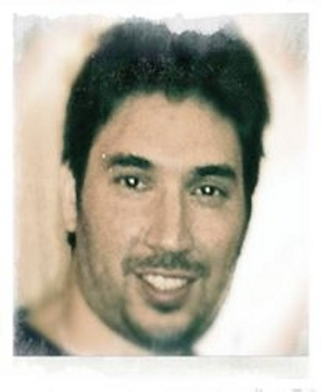
\includegraphics[width=0.15\textwidth]{photo}
%\end{wrapfigure}

%%% Photo
\begin{figure}
	\hfill
	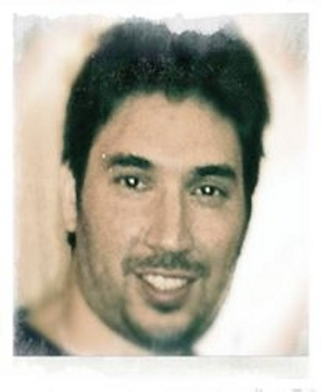
\includegraphics[width=0.2\textwidth]{photo}
	\vspace{-7cm}
\end{figure}

%%% Title
\MyName{Dario Palminio}
\MySlogan{Curriculum Vitae}

\sepspace

%%% Personal details
%%% ------------------------------------------------------------
\NewPart{Datos personales}{}

\PersonalEntry{Nacimiento}{6 de Enero de 1977}
\PersonalEntry{Localización}{5000 Cordoba, Argentina}
\PersonalEntry{Teléfono}{(000) 000-0000}
\PersonalEntry{Mail}{\url{dario.palminio@gmail.com}}
\PersonalEntry{Sitio web}{\url{https://www.palminio.com}}
\PersonalEntry{linkedin}{\url{https://www.linkedin.com/in/palminio}}
\PersonalEntry{CScrumMaster}{\url{https://www.scrumalliance.org/community/profile/dpalminio}}

%%% Education
%%% ------------------------------------------------------------
\NewPart{Educación}{}

%2003 - Systems Engineer: School of Exact Sciences, UNPA-UACO National University. Graduated in 2003.
\EducationEntry{Ingeniero de Sistemas}{2003}{UNPA-UACO}
{Universidad Nacional de la Patagonia Austral - Unidad Académica Caleta Olivia}
\sepspace

%2000, Analyst: University Analyst Programmer: School of Engineering, UNPSJB University National. Graduated in 2000.
\EducationEntry{Analista de Sistemas}{2000}{UNPSJB}
{University National de la Patagonia San Juan Bosco}
\sepspace

%1995, Electromechanical: Electromechanical technician: School ENET 1. Graduated in 1995.
\EducationEntry{Electromecánico}{1995}{ENET 1}
{Técnico mecánico eletricista}
\sepspace

%%% Work experience
%%% ------------------------------------------------------------
\NewPart{Experiencia laboral}{}

%2014-2015 Globant (globant.com) Software Engineer.
\WorkEntry{Globant}{2015-actual}{Technical Leader, Focal point y Java developer}
{1) Technical Lead en Perl/Java tecnologías para cuenta de LAN en empresa Globant. Las tecnologías usadas fueron: Perl (POO with Moose, cgi, Test::Moore, Template Toolkit), MySQL, Linux, SVN, Git-Svn, CSS3, HTML5, Eclipse (RSE, EPIC), Review Board, Jenkins, etc. The Java Technologies used was SOAP, RESTful/RESTEasy, Spring, Maven, Javascript with front-end using MVC (Backbone.js). Los proyectos fueron  relacionados a recolección de datos para envío a Google Analytic, gestión de promosiones y gestión de canje preferente de pasajes y usuarios Lanpass.
2) Focal point y Desarrollador Java en proyectos de cambio de pasajes con arquitectura SOA.}

\sepspace

%2012-2014 IBA Entertainment limited as Software Engineer Freelancer.
\WorkEntry{IBA Entertainment limited}{2012-2014}{Software Engineer Freelancer}
{Ingeniero de Software (como Freelancer/Monotributista) en tecnologías Perl para sistema de sportsbetting (Bet3000.com). Algunas tecnologías usadas: Perl 5, EmbPerl Object, Object Perl, JSON, RESTful, Mojolicious, Perl DBI. Desarrollo en el proyecto Bet3000 (www.bet3000.com) para la empresa International Betting Association.}

\sepspace

%2013-2014 Make IT Coop. As Associate, Secretary
\WorkEntry{Make IT Coop.}{2013-2014}{Associate, Secretary}{
Socio fundador y Secretario en Cooperativa Make IT Coop. También desarrollo en diferentes tecnologías web.}

\sepspace

%2008-2010 Motorola Mobility as Software Engineer.
\WorkEntry{Motorola Mobility}{2008-2010}{Software Engineer}
{Ingeniero de Software en desarrollos Java (J2EE para dispositivos móviles y sistema de telecomunicaciones) en Motorola Mobility de Argentina S.A.}

\sepspace

%2008-2010 Motorola S.C.A (Contractor Vates) as Software Engineer.
\WorkEntry{Motorola S.C.A (Contractor Vates)}{2008-2010}{Software Engineer}
{Desarrollador Java (J2SE and J2EE para dispositivos móviles y sistema de telecomunicaciones)}

\sepspace

%2008 Vates (www.vates.com) as Systems Engineer.
\WorkEntry{Vates}{2008}{Systems Engineer}
{Desarrollador Java para sistema de Gestión de Compras Municipal.}

\sepspace

%2007 Santex America S.A. (santexgroup.com) as Software Engineer: Java Developer.
\WorkEntry{Santex America S.A.}{2007}{Software Engineer, Java Developer}
{1) Desarrollador Java para sistema de Gestión de Procesos de Negocio.}

\sepspace

%2007 AYI & Asociados (BADI S.R.L) as Software Engineer: Java Developer, Computer Consultant Java.
\WorkEntry{AYI and Asociados (BADI S.R.L)}{2007}{Software Engineer, Java Developer, Computer Consultant Java}
{1) Desarrollador Java (J2EE) y Oracle para proyecto de Tarjeta Naranja.
2) Capacitador de "Oracle 9i: Build J2EE Applications" en InMotion, Santiago de Chile (Chile);
3) Capacitador de "Oracle AS 10g: R3 Build J2EE Applications" en oficinas de Oracle, Buenos Aires (Arg.).
}

\sepspace

%2006 Informatic forensics – Tribunal third in Comodoro Rivadavia City: Informatic Forensics.
\WorkEntry{Tribunal tercero de Comodoro Rivadavia}{2006}{Informático Forense}{
Informático Forense para el tribunal tercero de Comodoro Rivadavia}

\sepspace

%2004-2006 24 months in Municipality of Comodoro Rivadavia city, Systems Engineer Juridical Informatics, Technical Leader.
\WorkEntry{Municipalidad de Comodoro Rivadavia}{2004-2006}{Systems Engineer Juridical Informatics, Technical Leader}
{Líder Técnico en Proyecto de Digesto Legislativo Municipal en Asesoría letrada de la Municipalidad de Comodoro Rivadavia.}

\sepspace

%2004-2005 Teacher Mathematic Teacher, Software Teacher, Computation Teacher.
\WorkEntry{Profesor}{2004-2005}{Teacher Mathematic Teacher, Software Teacher, Computation Teacher}
{Profesor: 
1- Computación I (Basic Informatic) - ISIS (Instituto terciario privado); 
2- Computación II (Aplicaciones de Software) - ISIS (Instituto terciario privado); 
3- Computación III (Linux y Windows Net) - ISIS (Instituto terciario privado); 
4- Profesor de Software: Adaptación al ambiente de trabajo en ENET 2 (Escuela Técnica); 
5- Profesor de Matemática de 8-EGB  (dos cursos)- Escuela 119 (C. R.); 
6- Profesor de Matemática de 9-EGB (dos cursos)- Escuela 119 (C. R.).
}

\sepspace

%2000-2003 - DeSoft Development of Software
\WorkEntry{DeSoft}{2000-2003}{Developer, Technical Leader}{
Desarrollador y Líder técnico en proyectos de desarrollo de software para empresas de terserización petrolera y máquinas viales.}

\sepspace

%%% Certifications
%%% ------------------------------------------------------------
\NewPart{Certificaciones}{}

\CertificatesEntry{\large{\textbf{ScrumMaster}}}{}
\CertificatesEntry{}{
Certified ScrumMaster por SCRUM ALLIANCE.\newline
Licencia: 000428099\newline
URL: \url{https://www.scrumalliance.org/community/profile/dpalminio}
}
\sepspace

\CertificatesEntry{\large{\textbf{SMAC}}}{}
\CertificatesEntry{}{
Scrum Master Accredited Certification por International Scrum Institute.\newline
Licencia: 59173583922442\newline
URL: \url{http://www.scrum-institute.org/International_Scrum_Institute_Certificate_Validation_Tool.php}
}
\sepspace

\CertificatesEntry{\large{\textbf{SPOAC}}}{}
\CertificatesEntry{}{
Scrum Product Owner Accredited Certification por International Scrum Institute.\newline
Licencia: 92432962027378\newline
URL: \url{http://www.scrum-institute.org/International_Scrum_Institute_Certificate_Validation_Tool.php}
}
\sepspace

\CertificatesEntry{\large{\textbf{SC4JD}}}{}
\CertificatesEntry{}{
Scrum Certification for Java Developer por International Scrum Institute.\newline
Licencia: 96122926946263\newline
URL: \url{http://www.scrum-institute.org/International_Scrum_Institute_Certificate_Validation_Tool.php}
}
\sepspace

%%% Courses
%%% ------------------------------------------------------------
\NewPart{Cursos de Gestión y Organización}{}

\CoursesEntry{Curso de Certified Scrum Master}{2015}{Kleer, Cba.-Arg.}{}
\CoursesEntry{Especialización en Project Management}{2010}{UTNFRBA, Bs.As.-Arg.}{}
\CoursesEntry{Carrera de Project Management}{2008}{IAAP, PMI, Bs.As.-Arg.}{}
\CoursesEntry{Estructuración de Proyectos PM01.}{2007}{IAAP, Bs.As.-Arg.}{}
\CoursesEntry{Creación de Cooperativas.}{2012}{INAES, Cba.-Arg.}{}

\sepspace

%%% Skills - Otras Experiencias y Conocimientos
%%% ------------------------------------------------------------
\NewPart{Otras Experiencias y Conocimientos}{}

\sepspace

\SkillsEntry{\textbf{Languages}}{Spanish (mother tongue)}
\SkillsEntry{}{English (level 2)}

\sepspace

\SkillsEntry{Software}{
\textsc{Java}, \LaTeX, \textsc{Perl}, \textsc{MySQL}, etc.
}


%%% References
%%% ------------------------------------------------------------
\NewPart{Referencias}{}
Para más información ver el prefil en linkedin.

\sepspace

\end{document}
